% ||||||||||||||||||||||||||||||||||||||||||||||
% Capitulo de Resultados Preliminares
% ||||||||||||||||||||||||||||||||||||||||||||||

\chapter{Análine de Resultados}

Nesse capítulo são apresentados os resultados preliminares das técnicas desenvolvidas, mostrando a viabilidade das mesmas. Os resultados 
foram descritos na mesma sequência que foram estudados no capítulo de revisão bibliográfica.


%++++++++++++++++++++++++++++++++++++++++++++++++++++++++++++++++
% 
%++++++++++++++++++++++++++++++++++++++++++++++++++++++++++++++++

\subsection{Análise dos Resultados de Campo}


\begin{figure}[H]
    \caption{Linhas de base e sinais coletados do eixo x.}
    \begin{center}
        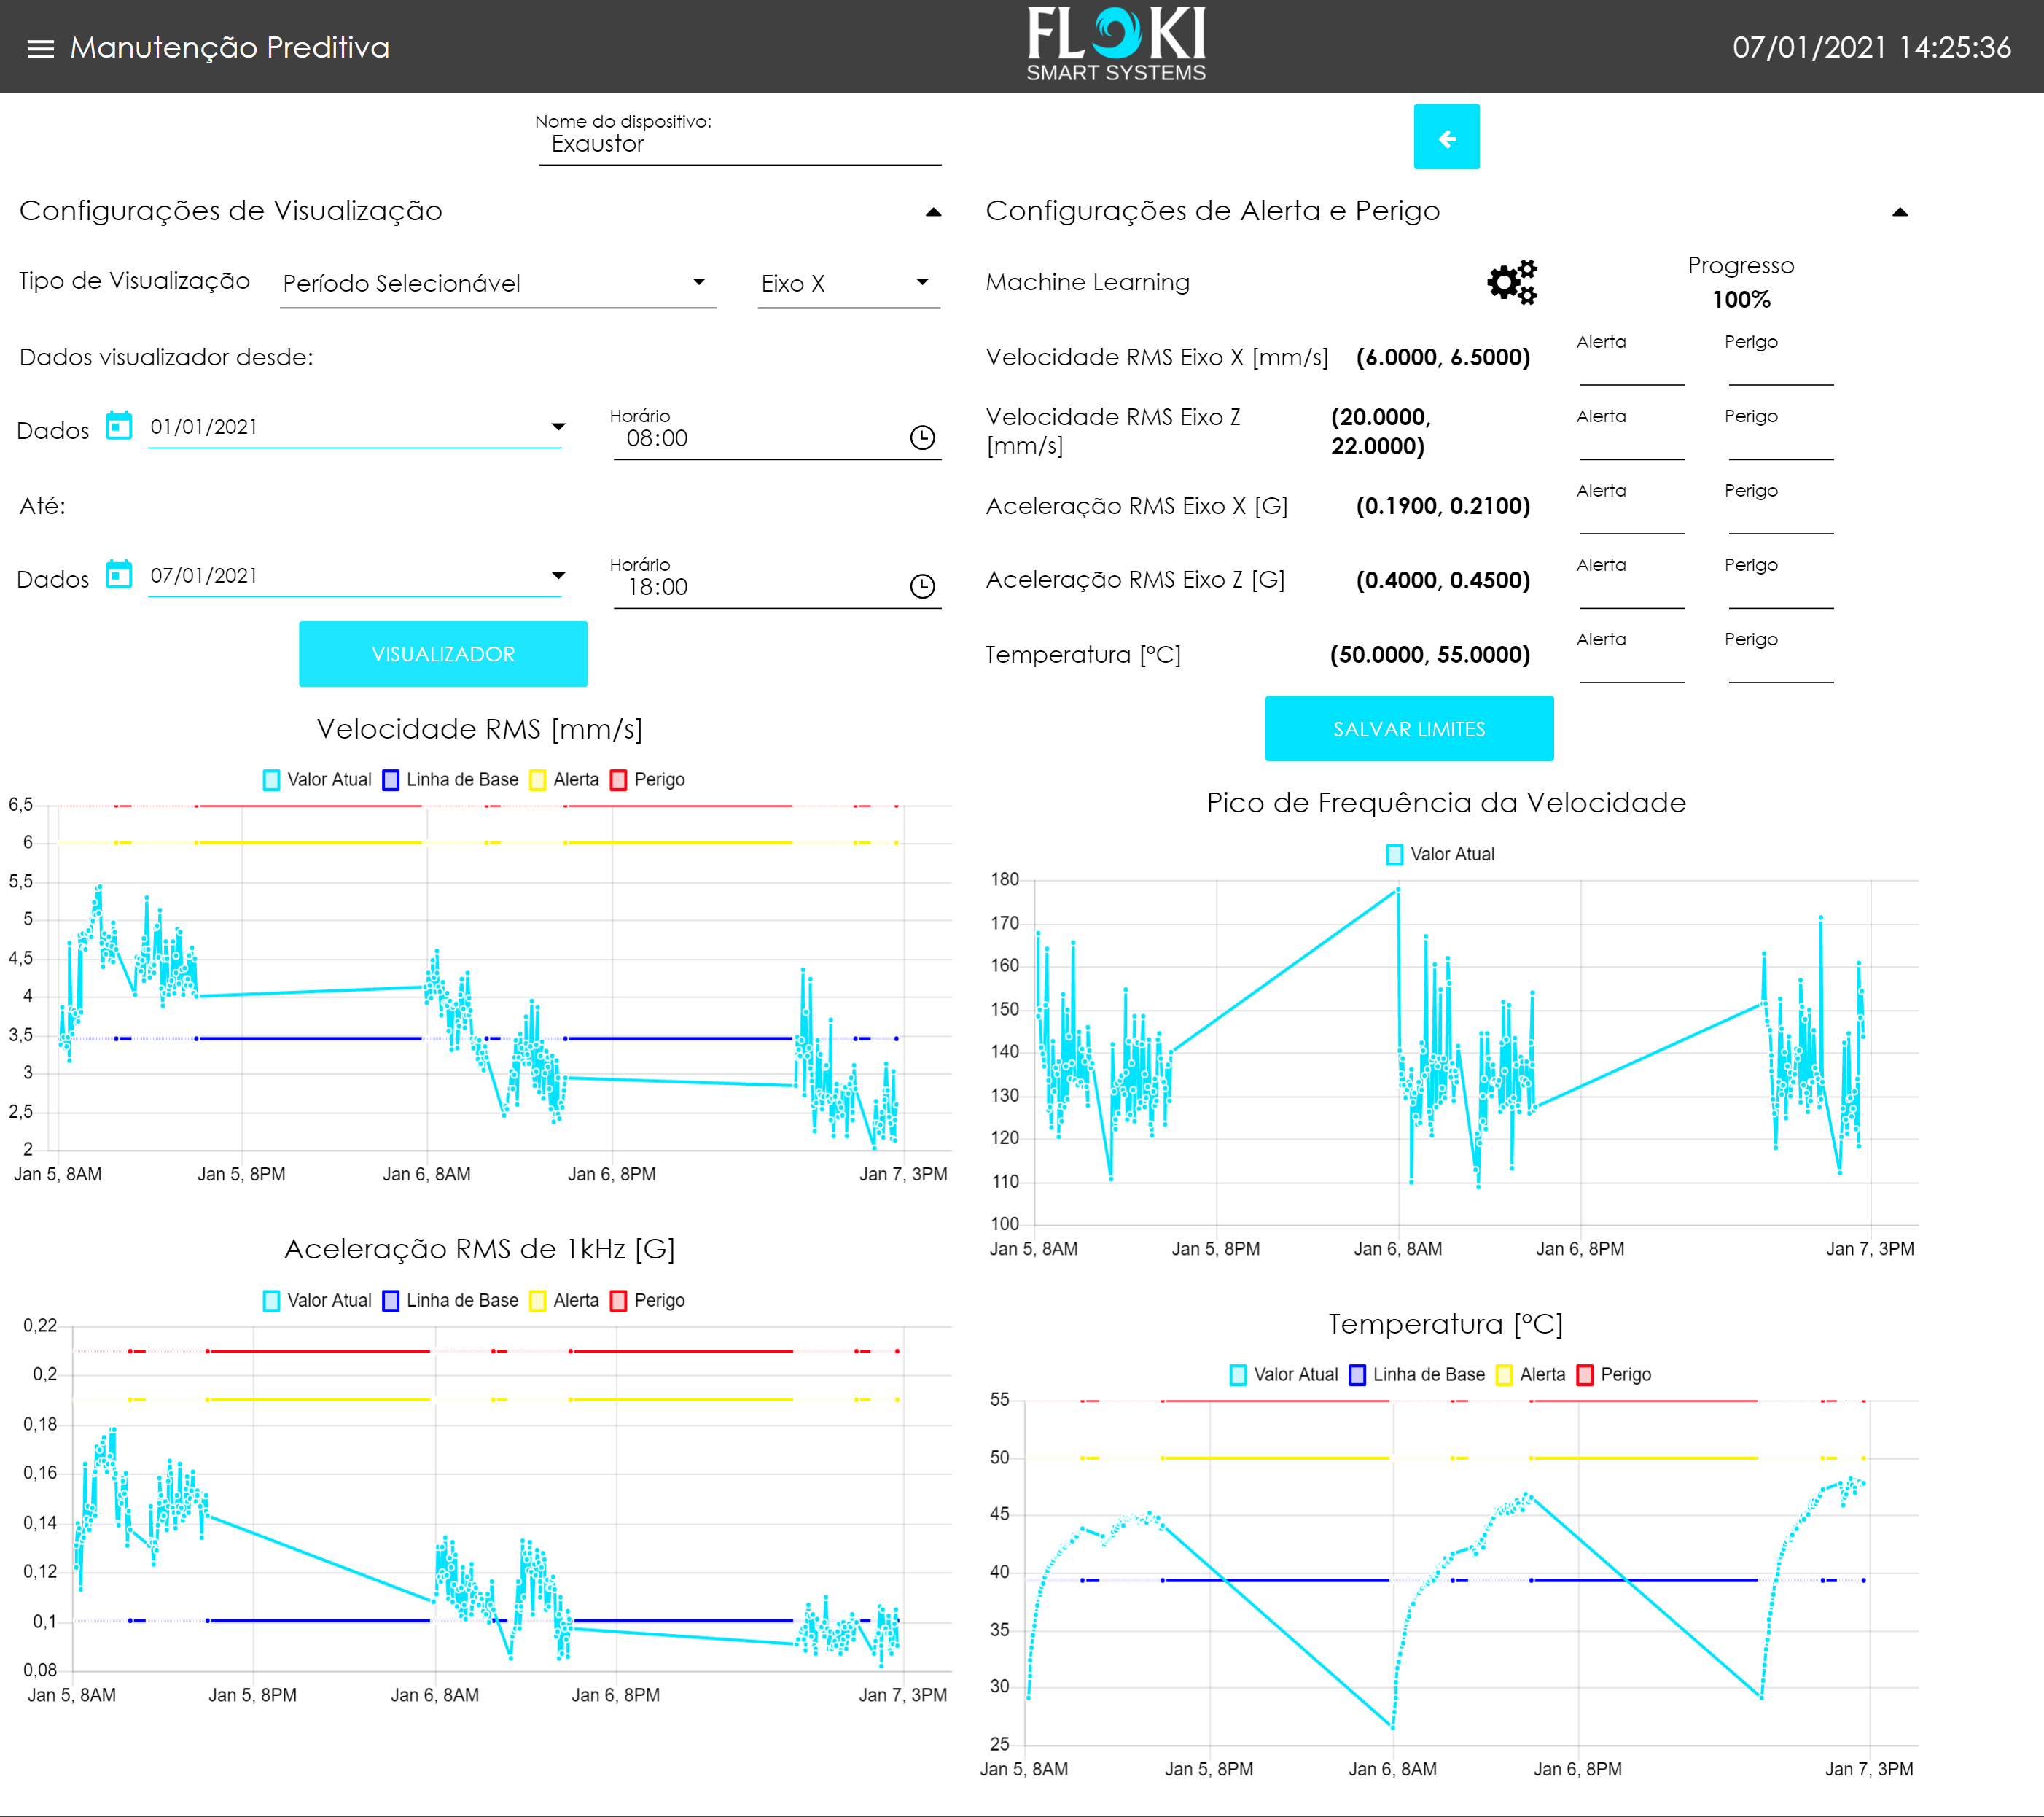
\includegraphics[scale=.15]{resultados/img/drakkar_eixo_x.png}
    \end{center}
    \fonte{Elaborado pelo Autor.} 
    \label{fig:ica}
\end{figure}

\begin{figure}[H]
    \caption{Linhas de base e sinais coletados do eixo z.}
    \begin{center}
        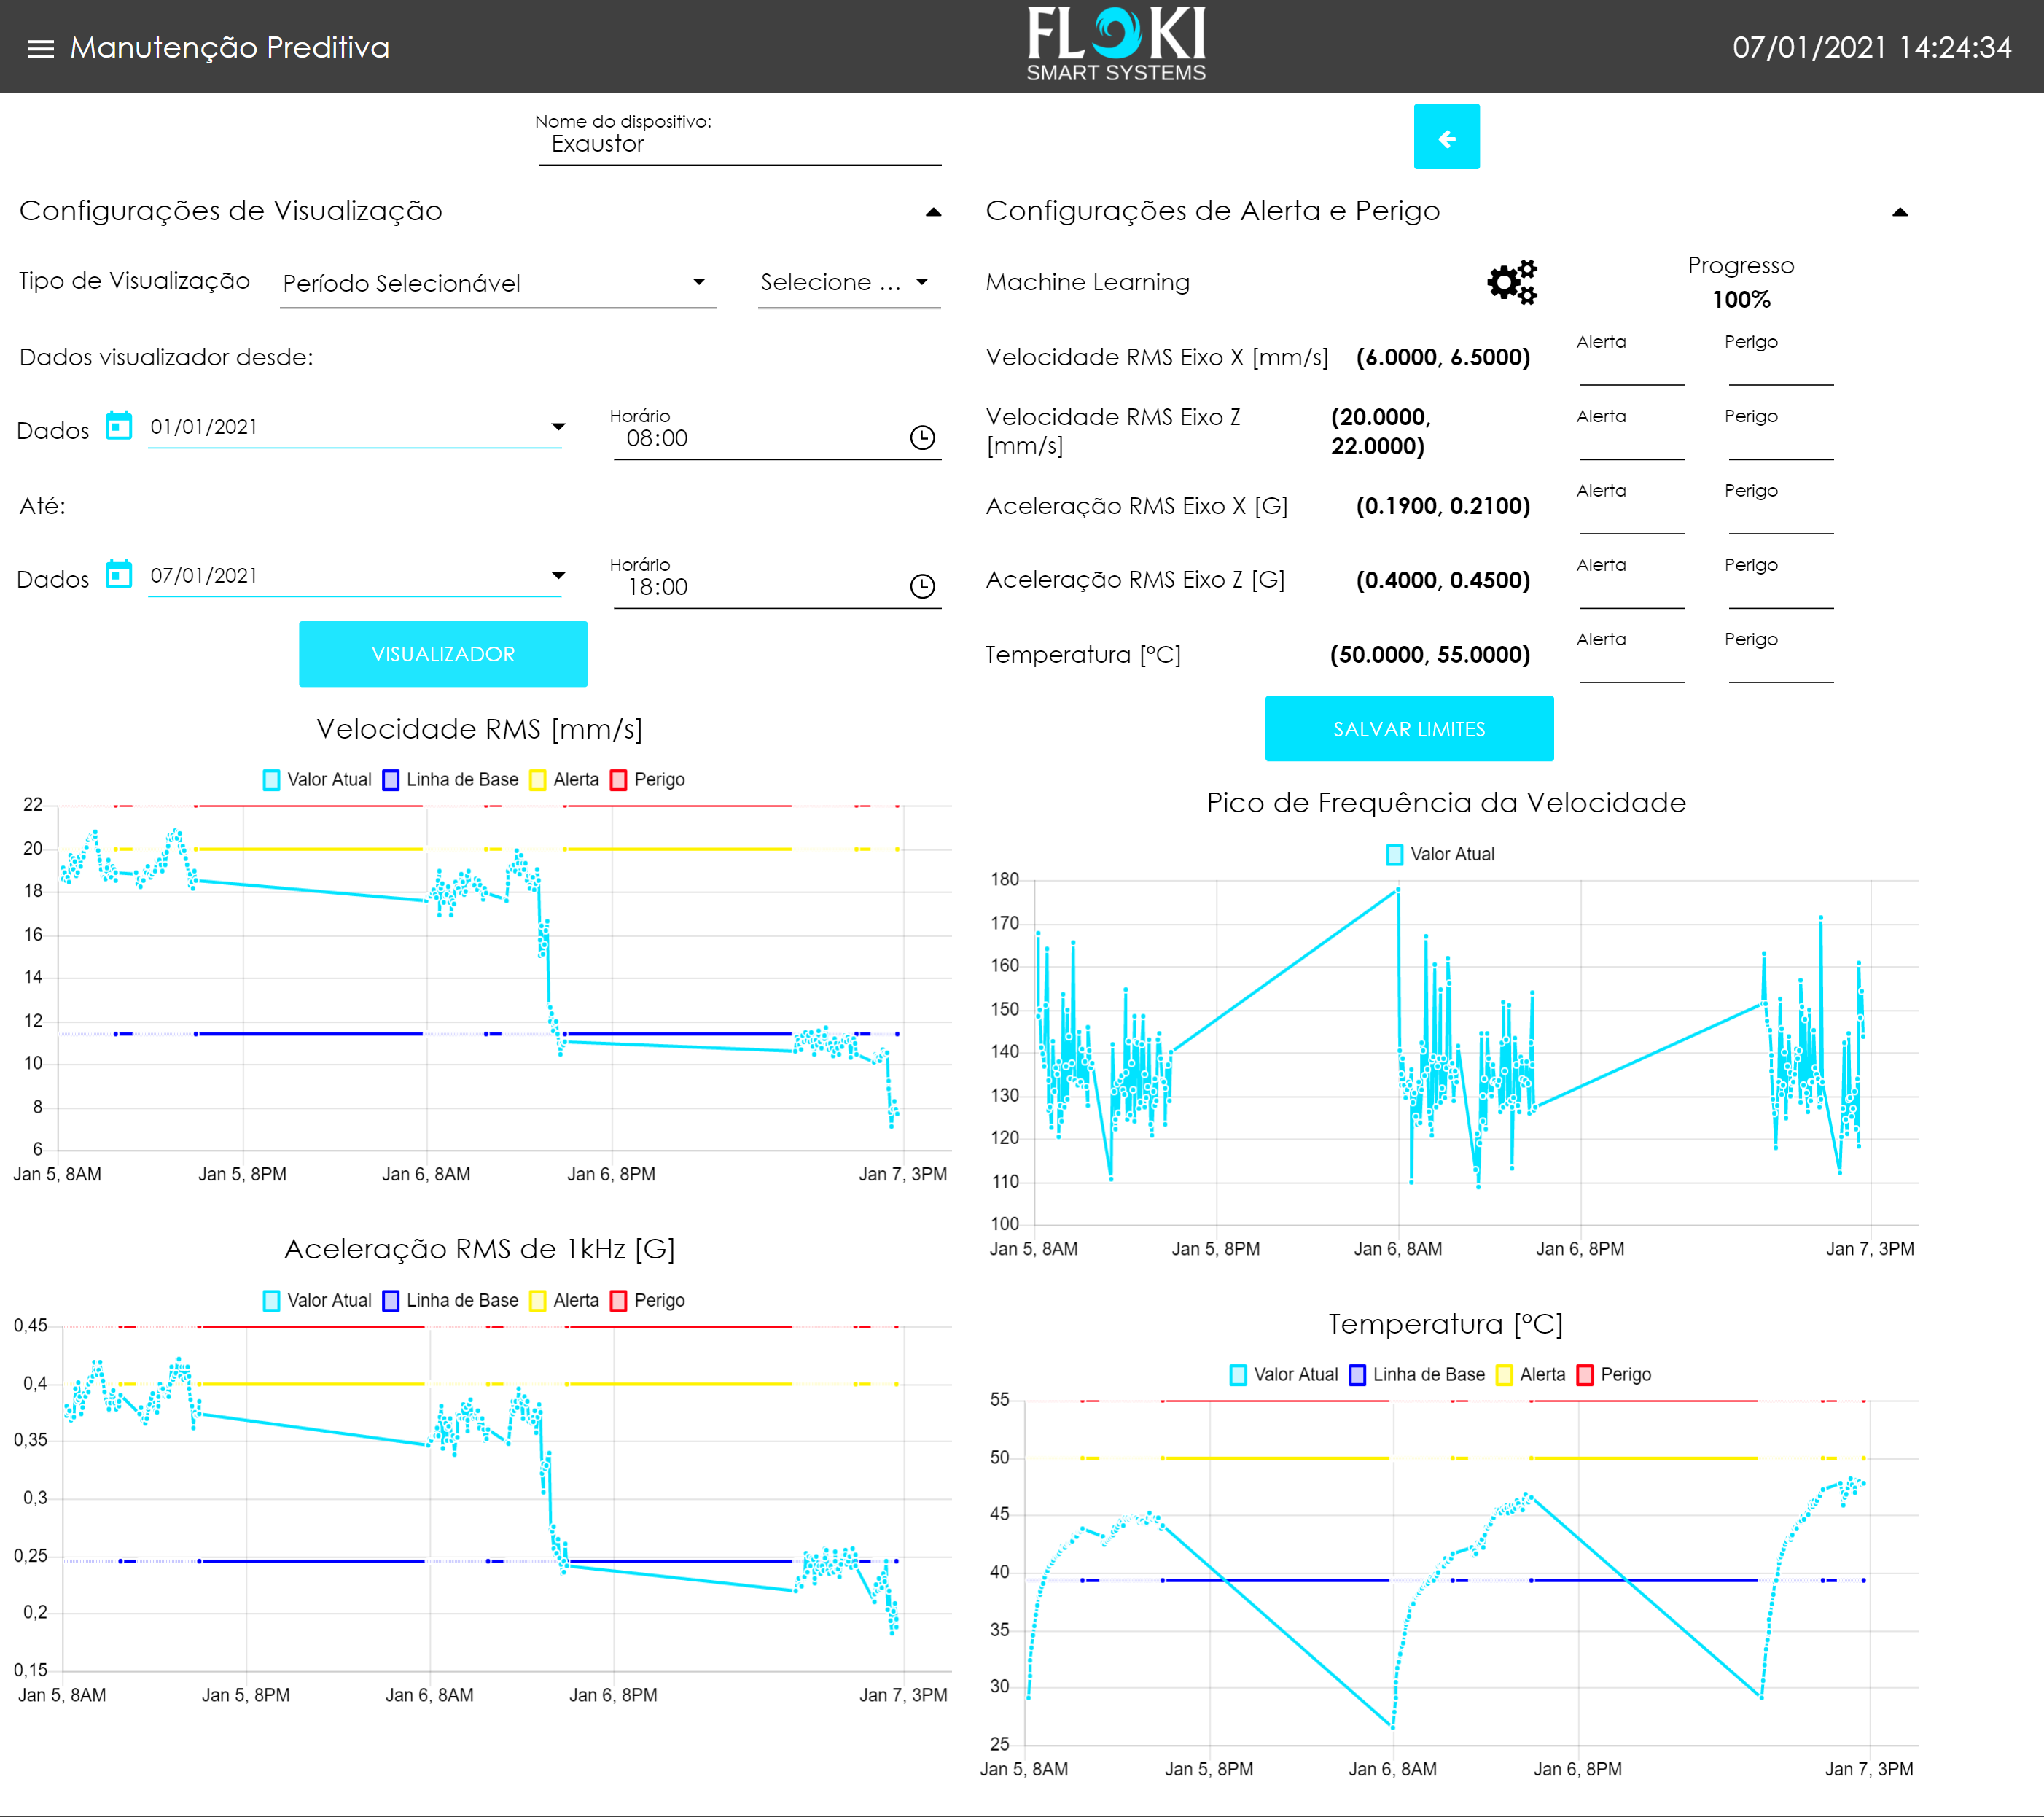
\includegraphics[scale=.15]{resultados/img/drakkar_eixo_y.png}
    \end{center}
    \fonte{Elaborado pelo Autor.} 
    \label{fig:ica}
\end{figure}

Como podemos ver, o eixo Z se encontra em estado severo de vibração, não entrando em alarme devido ao ajuste manual do operador da fábrica,
sendo agora um problema humano realizar as tarefas de forma correta.


Após a escrita de todo o trabalho, indo desde o conhecimento mínimo para o entendimento das propostas, passando pela descrição dos métodos
empregados, até os resultados preliminares, foi possível ver o funcionamento satisfatório das técnicas, mas que ainda precisam de melhorias
e a aplicação de uma CNN para classificar os resultados até agora obtidos. 

